\label{sec:mtproto2-informal}

In this chapter, we will give a brief overview of the MTProto2.0 protocol. A more in-depth and formal description can be found on the official web page \cite{Telegram-MTProto2.0}.

First of all, MTProto2.0 is a \textit{suite of protocols} used to enable secure communication between a Telegram client and a Telegram server over an insecure network. MTProto2.0 can be decomposed in the three following protocols:

\begin{description}[style=nextline]
  \item[Authorization] used to obtain a secret authorization key shared only with the server;
  \item[\Schat{}] used to obtain a secret key shared between two clients. This is then used to exchange end-to-end messages between two clients, with the server that basically acts as a forwarder;
  \item[Rekeying] used to achieve \pfs{}, allows obtaining a new end-to-end encryption key.
\end{description}

Additionally, the \cchats{} encryption schema is used to securely exchange messages between clients and servers (who have shared an authorization key).

An overview on these protocols will be given in \cref{sec:auth-prot,sec:cloud-chat,sec:secret-chat,sec:rekeying}.

\section{Authorization protocol}
\label{sec:auth-prot}

%% Authorization protocol %%
\begin{figure}[!t]
  \setlength{\instdist}{4cm}
  \setmscoptions
  \begin{msc}{}
    \setmscscale{.8}

    \declinst{client}{}{Client}
    \declinst{server}{}{Server}

    \action*{Generates nonces $n_{c}, n_{k}$}{client}
    \action*{\parbox{4.5cm}{\centering
        Knows keys $\mbox{sk}^{(1)}, \dots, \mbox{sk}^{(n)}$\\
        Generates $n_s, g, p$\\
        Generates proof-of-work primes $q, r$
      }}{server}
    \nextlevel[6]

    \mess{$n_{c}$}{client}{server}
    \nextlevel[2]
    \mess{$n_{c}, n_{s}, q \cdot r, \mbox{fp}^{(1)}, \dots, \mbox{fp}^{(n)}$}{server}{client}

    \nextlevel
    \action*{\parbox{4cm}{\centering
        Chooses $\mbox{pk}^{(i)}$ matching\\
        $\mbox{fp}^{(i)}$ for some $i$\\
        Factorizes $q \cdot r$\\
        $C_1 := q \cdot r, q, r, n_c, n_s, n_k$
      }}{client}

    \nextlevel[7]
    \mess{$n_c, n_s, q, r, \mbox{fp}^{(i)}, \enc{\sha{1}{C_1}, C_1}{\mbox{pk}^{(i)}}$}{client}{server}
    \nextlevel

    \action*{$\left(k, iv\right) := \kdf{n_s, n_k}$}{client}
    \action*{\parbox{4.5cm}{\centering
        $s \in \group{p}$\\
        $g_s := \modexp{g}{s}{p}$\\
        $key, iv := \kdf{n_s, n_k}$\\
        $S_1 := n_c, n_s, g, p, g_s, t_1$
      }}{server}

    \nextlevel[6]
    \mess{$n_c, n_s, \enc{\sha{1}{S_1}, S_1}{key, iv}$}{server}{client}
    \nextlevel

    \action*{\parbox{4.5cm}{\centering
        $c \in \group{p}$\\
        $g_c := \modexp{g}{c}{p}$\\
        Checks $g, p$\\
        $\key{CS} := \modexp{g_s}{c}{p}$\\
        $C_2 := n_c, n_s, retryID, g_c$
      }}{client}
    \nextlevel[7]

    \mess{$n_c, n_s, \enc{\sha{1}{C_2}, C_2}{k, iv}$}{client}{server}
    \nextlevel

    \action*{\parbox{4.5cm}{\centering
        $\key{CS} := \modexp{g_c}{s}{p}$
      }}{server}
    \nextlevel[3]

    \mess{$n_c, n_s, \hash{n_k, \key{CS}}$}{server}{client}


  \end{msc}
  \centering
  \caption{MTProto2.0 Authorization protocol}
  \label{fig:authorization-protocol}
\end{figure}


The first time a Telegram client C runs the application, it must negotiate an \textbf{authorization key} with the Telegram server S. The authorization protocol is used to this end. Once the client and the server have shared an authorization key, they will use it to encrypt (almost) every future communication between them. A client might also have several keys (e.g. on multiple devices or if reinstalling the application), some of which might be locked (e.g. if the device is lost). The authorization protocol is based on the \DiHe{} key exchange protocol \cite{DH-protocol}.


A successful protocol run consists of three rounds, which are represented schematically in \cref{fig:authorization-protocol}:
\begin{description}
  \item[Round 1] In the first round, messages are in plaintext. In particular, the client and the server exchange two nonces ($n_c$ and $n_s$). The pair $\left<n_c, n_s\right>$ identifies a session of the authorization protocol. These nonces are sent in every consequent message of the current run of the protocol, both in plaintext and encrypted form.
    \begin{enumerate}
      \item{In the first message, the client sends his fresh nonce $n_c$ to the server;}
      \item{The server answers with the client nonce $n_c$, the server fresh nonce $n_s$, a challenge $q \cdot r \leq 2^{63}$ (which are two primes used as a measure to prevent denial of service, as the client needs to spend resources on factorizing $q \cdot r$ before the server has to commit (more) resources\footnote{Notice that this might not be true as this might be vulnerable to a lookup table approach (e.g. using \href{http://factordb.com}{factordb.com}).}) and a list of public RSA key fingerprints (calculated as the lower 64-bits of the SHA1 of the server public keys).}
    \end{enumerate}

  \item[Round 2] The client decomposes $q\cdot r$ in $\left<q, r\right>$ and retrieves the public key of the server $pk^{\left(i\right)}$. The client then generates a nonce $n_k$ of 256 bits. This nonce $n_k$ is supposed to be secret. The pair $\left<n_s, n_k\right>$ is used, by both server and client, to derive, through a derivation function $\mbox{kdf}$, a symmetric encryption key $k$ and an initialization vector $iv$, which will be used in subsequent exchanges.
    \begin{enumerate}
      \setcounter{enumi}{2}
      \item{The client asymmetrically encrypts both $\left<q\cdot r, q, r, n_c, n_s, n_k\right>$ and its SHA1 hash with $pk^{(i)}$ and sends it along with $\left<n_c, n_s, q, r, fp^{(i)}\right>$ to the server. A rather complex padding schema is used;}
      \item{The server generates his \DiHe{} ephemeral key $s$ of 2048-bits, chooses $g, p$ and computes $g_s:= \modexp{g}{s}{p}$. Finally, it symmetrically encrypts both $\left<n_c, n_s, g, p, g_s, t_1\right>$ and its SHA1 hash and sends it along with $\left<n_c, n_s\right>$.}
    \end{enumerate}

    Notice that the client is supposed to check that:
    \begin{itemize}
      \label{item:DH-clients-checks}
      \item{$p$ is a safe 2048-bit prime, where safe means that both $p$ and $\frac{p-1}{2}$ are prime and $2^{2047} < p < 2^{2048}$;}
      \item{$g$ is a generator for $\frac{p-1}{2}$.}
    \end{itemize}

  \item[Round 3] In the last round, the client generates his own \DiHe{} ephemeral key and shares it with the server.
    \begin{enumerate}
      \setcounter{enumi}{4}
      \item{The client generates his ephemeral key $c$ of 2048-bits and computes $g_c:= \modexp{g}{c}{p}$. Then, it symmetrically encrypts both $\left<n_c, n_s, retryID, g_c\right>$ and its SHA1 hash and sends them along with $\left<n_c, n_s\right>$. The $retryID$ starts at zero at the time of the first attempt, otherwise is based on the values from the last failed attempt;}
      \item{The server is now able to compute the authorization key as $\key{CS}:= \modexp{g_c}{s}{p}$. Assuming server checks pass, S sends an acknowledgment for the new key: $\left<n_c, n_s, \hash{\key{CS}}\right>$.}
    \end{enumerate}

\end{description}


\section{\Cchat{} encryption schema}
\label{sec:cloud-chat}

%% Cloud-chat encryption schema %%
\begin{figure}[t]
  \centering
  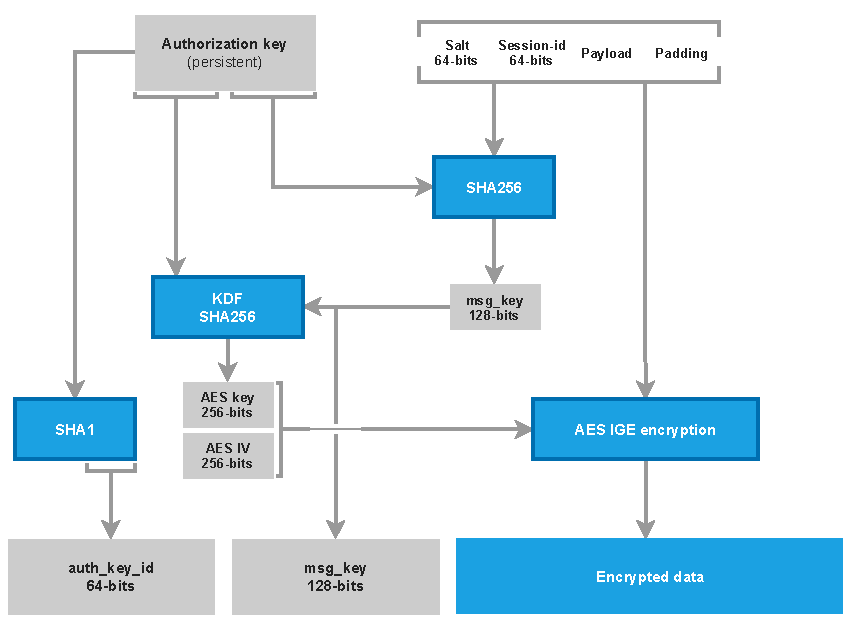
\includegraphics{cloud-chats}
  \caption{MTProto2.0 \cchat{} protocol.\\Representation inspired by the Telegram's official one.}
  \label{fig:cloud-chat-protocol}
\end{figure}
\begin{figure}[t]
  \centering
  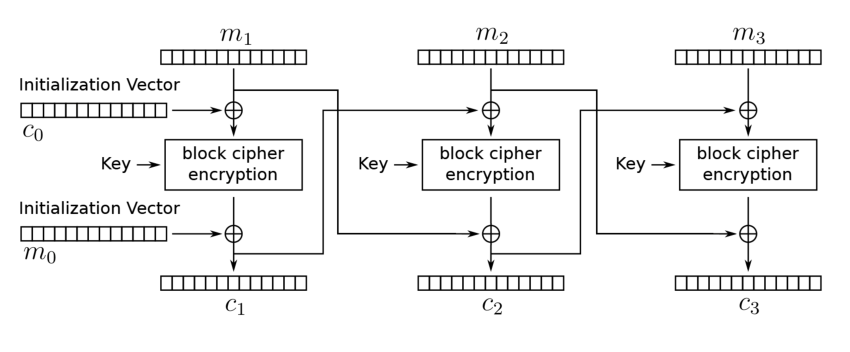
\includegraphics{IGE}
  \caption{Encryption in IGE mode.}
  \label{fig:IGE}
\end{figure}

Telegram uses the schema in \cref{fig:cloud-chat-protocol} to encrypt every message exchanged between the client and the server after an authorization key has been established using the authorization protocol in \cref{sec:auth-prot}.

A message key msg\_key of 128 bits is calculated as the middle 128 bits of the SHA256 of the entire message prepended by 32 bytes of the authorization key. The message itself contains a 64-bit salt, a 64-bit session identifier, the payload\footnote{The payload contains the time of the message, its length, a sequence number. The receiver should check these pieces of information after decryption.} and a variable size padding of 12-1024 bytes.
The authorization key auth\_key, combined with the message key msg\_key, is used to derive a key and an initialization vector, which are used to encrypt the entire message using AES in IGE mode.

\subsection{IGE mode}
Infinite Garble Extension (in short, IGE) is a block cipher mode, lesser-known than others like ECB, CBC, OFB, CTR, CFB, GCM, CCM.
IGE can be defined with the following formula:

\begin{equation}
  c_i = f_K(m_i \oplus c_{i-1}) \oplus m_{i-1}
\end{equation}

where $f_K$ stands for the encrypting function (like AES) with key $K$
and $i$ goes from 1 to $n$ (the number of plaintext blocks). Two initialization vectors, $c_0$ and $m_0$, are also needed. \Cref{fig:IGE} summarizes how the encryption in IGE mode works.


One of the main properties of IGE mode is that it makes sure that if a ciphertext block is changed, then every subsequent block following it will not decrypt correctly.

As pointed out by \cite{Telegram-AFAQ-IGE}, the Telegram developers team is aware of the vulnerability of this mode to blockwise-adaptive Chosen Plaintext Attack (CPA)\cite{IGE-CPA}, but they claim that MTProto2.0 is not affected.




\section{\Schat{} protocol}
\label{sec:secret-chat}

Telegram's \schats{} deal with end-to-end encryption between two clients (as usual, let us call the clients Alice and Bob, or A and B for brevity). After both clients have shared an authorization key with the Telegram server S, they can decide to engage themselves in a run of the \schat{} protocol, allowing them to share, using a \DiHe{} key exchange, a common secret. Notice that the server acts as a forwarder: every message sent from a client A to another client B is sent to the server, encrypted as a \cchat{} message shown in \cref{sec:cloud-chat} with the authorization key of A; the server then decrypts the message and encrypts it as a \cchat{} message using the authorization key of B and finally sends it to B. The writing $\enc{M}{\key{AS}}$ in \cref{fig:secret-chat-protocol} expresses that the message $M$ has been encrypted with the authorization key $\key{AS}$ using the \cchat{} encryption schema \cref{sec:cloud-chat}.

%% Secret-chat protocol %%
\begin{figure}[!t]
  \setlength{\instdist}{3cm}
  \setmscoptions
  \begin{msc}{}
    \setmscscale{.8}

    \declinst{alice}{}{Alice}
    \declinst{server}{}{Server}
    \declinst{bob}{}{Bob}

    % Initial knowledge (auth keys)
    \action*{Knows $\key{AS}, \key{BS}$}{server}
    \action*{Knows $\key{AS}$}{alice}
    \action*{Knows $\key{BS}$}{bob}

    \nextlevel[3]
    \mess{$\enc{\func{getDhConfig}{}}{\key{AS}}$}{alice}{server}
    \nextlevel[2]
    \mess{$\enc{g, p}{\key{AS}}$}{server}{alice}
    \nextlevel

    \action*{\parbox{4cm}{\centering
        Generates $sID$\\
        $a \in \group{p}$\\
        $g_a := \modexp{g}{a}{p}$
      }}{alice}

    \nextlevel[5]

    %% TODO: Telegram webpage does not seem to specify HOW this is encrypted!!
    %% UPDATE: It actually (kinda) does: it's encrypted as a cloud-chat message! For simplicity, keep this notation and explain its meaning in the written part.
    \mess{$\enc{sID, B, g_a}{\key{AS}}$}{alice}{server}
    \nextlevel
    \mess{$\enc{sID, B, A, g_a}{\key{BS}}$}{server}{bob}
    \nextlevel[2]
    \mess{$\enc{\func{acceptChat}{}}{\key{BS}}$}{bob}{server}
    \nextlevel[2]
    \mess{$\enc{g, p}{\key{BS}}$}{server}{bob}
    \nextlevel

    \action*{\parbox{4cm}{\centering
        $b \in \group{p}$\\
        $g_b := \modexp{g}{b}{p}$\\
        $\key{AB} := \modexp{g_a}{b}{p}$
      }}{bob}

    \nextlevel[5]
    \mess{$\enc{sID, g_b, \sha{1}{k_{AB}}}{\key{BS}}$}{bob}{server}
    \nextlevel
    \mess{$\enc{sID, B, g_b, \sha{1}{k_{AB}}}{\key{AS}}$}{server}{alice}
    \nextlevel

    \action*{\parbox{4cm}{\centering
        $\key{AB} := \modexp{g_b}{a}{p}$\\
        Generates $msg$
      }}{alice}

    \nextlevel[3]
    \condition{Out-of-band $\key{AB}$ fingerprint comparison}{alice,server,bob}
    \nextlevel[4]
    \mess{$\enc{\enc{msg}{\key{AB}}}{\key{AS}}$}{alice}{server}
    \nextlevel
    \mess{$\enc{\enc{msg}{\key{AB}}}{\key{BS}}$}{server}{bob}

  \end{msc}

  \centering
  \caption{MTProto2.0 \Schat{} protocol}
  \label{fig:secret-chat-protocol}
\end{figure}

Let us describe the protocol steps, which are summed up in \cref{fig:secret-chat-protocol}. We will examine a run where Alice requests the \schat{}. Notice that we assume that both Alice and Bob have already exchanged an authorization key with the server ($\key{AS}$ and $\key{BS}$, respectively).

\begin{enumerate}
  \item{First of all, client A retrieves \DiHe{} parameters ($p, g$) from the server. Then, it generates a \DiHe{} ephemeral key $a$ and a session identifier $sID$. Finally, it computes his \DiHe{} half key $g_a:= \modexp{g}{a}{p}$ and sends $\left<sID, B, g_a\right>$ to client B;}
  \item{Client B receives the \schat{} request and may either accept it or deny it. Upon accepting it, it receives $p, g$, generates his ephemeral key $b$, computes his half key $g_b:= \modexp{g}{b}{p}$ and the newly created \schat{} key $\key{AB}:= \modexp{g_a}{b}{p}$. Lastly, it sends $\left<sID, g_b, \sha{1}{\key{AB}}\right>$ to client A. The hash function performed on the key is, as stated in the official documentation, only used as a sanity check for client developers;}
  \item{Client A receives the half key of B $g_b$ and uses it to compute the \schat{} key $\key{AB}:= \modexp{g_b}{a}{p}$. If the fingerprint of the key matches the one sent by B, it accepts the \schat{} and can start sending and receiving messages\footnote{The encryption schema used to encrypt end-to-end messages is very similar to the \cchat{} schema. We will not report it for brevity. The main difference is in the composition of the message. Please refer to \cite{Telegram-EndToEnd} for more details.}.}
\end{enumerate}

Mind that \DiHe{} generator ($g$), ephemeral keys ($a, b$) and half keys ($g_a, g_b$) are supposed to be checked by the clients as shown in \cref{item:DH-clients-checks}. Additionally, they should check all these values are greater then $1$ and smaller then $p-1$. Telegram team also recommends to check that $2^{2048}\leq g_a, g_b \leq \left(p-2\right)^{2064}$.

Notice that, as this exchange lacks authentication of the two clients, a compromised server can trivially perform a classic \DiHe{} \mitm{} attack \cite{DH-MITM}. To this end, Telegram requires the clients to check if their key fingerprints match. This must be done in an authenticated way using an out-of-band channel (e.g. in-person). This comparison is a necessary condition to ensure secrecy in further exchanges between participating clients.

\section{Rekeying protocol}
\label{sec:rekeying}

%% Rekeying protocol %%
\begin{figure}[t]
  \setlength{\instdist}{3.5cm}
  \setmscoptions
  \begin{msc}{}
    \setmscscale{.8}

    \declinst{alice}{}{Alice}
    \declinst{server}{}{Server}
    \declinst{bob}{}{Bob}

    % Initial knowledge (auth keys)
    \action*{Knows $\key{AS}, \key{BS}$}{server}
    \action*{Knows $\key{AS}, \key{AB}, p, g$}{alice}
    \action*{Knows $\key{BS}, \key{AB}, p, g$}{bob}

    \nextlevel[2]
    \action*{\parbox{4cm}{\centering
        Generates $eID$\\
        $a \in \group{p}$\\
        $g_a := \modexp{g}{a}{p}$
      }}{alice}

    \nextlevel[6]
    \mess{$\enc{\enc{eID, g_a}{\key{AB}}}{\key{AS}}$}{alice}{server}
    \nextlevel
    \mess{$\enc{\enc{eID, g_a}{\key{AB}}}{\key{BS}}$}{server}{bob}
    \nextlevel

    \action*{\parbox{4cm}{\centering
        $b \in \group{p}$\\
        $g_b := \modexp{g}{b}{p}$\\
        $\newkey{AB} := \modexp{g_a}{b}{p}$
      }}{bob}

    \nextlevel[6]
    \mess{$\enc{\enc{eID, g_b, \sha{1}{\newkey{AB}}}{\key{AB}}}{\key{BS}}$}{bob}{server}
    \nextlevel
    \mess{$\enc{\enc{eID, g_b, \sha{1}{\newkey{AB}}}{\key{AB}}}{\key{AS}}$}{server}{alice}
    \nextlevel

    \action*{\parbox{4cm}{\centering
        $\newkey{AB}:= \modexp{g_b}{a}{p}$
      }}{alice}

    \nextlevel[4]
    \mess{$\enc{\enc{eID, \sha{1}{\newkey{AB}}}{\key{AB}}}{\key{AS}}$}{alice}{server}
    \nextlevel
    \mess{$\enc{\enc{eID, \sha{1}{\newkey{AB}}}{\key{AB}}}{\key{BS}}$}{server}{bob}

  \end{msc}

  \centering
  \caption{MTProto2.0 Rekeying protocol}
  \label{fig:rekeying-protocol}
\end{figure}

This protocol is used to enable \pfs{} in \schats{}. Clients compliant with the protocol specification are supposed to initiate rekeying once a \schat{} key has been used to encrypt and decrypt more than 100 messages, or it has been in use for at least a week (and was used at least once). Any client participating in a \schat{} can start a run of the rekeying protocol.

Rekeying is based on \DiHe{}, which ensures that access to old keys does not grant knowledge of new ones. Moreover, the exchange is encrypted with the \schat{} key shared between clients, which effectively authenticates clients under the assumption of secrecy of the key itself. Under the premise of secrecy of the initial \schat{} key, this also rules out the possibility of a \mitm{} attack executed by a compromised server.

Let us examine the rekeying protocol, represented schematically in \cref{fig:rekeying-protocol}. We assume that clients engaging the rekeying protocol have already shared a \schat{} key $\key{AB}$. In addition, clients re-use \DiHe{} parameters $p, g$ obtained from the previous \schat{} protocol run.

\begin{enumerate}
  \item{Client A generates its \DiHe{} ephemeral key $a$ and an exchange identifier $eID$. Then, it computes its half key $g_a:= \modexp{g}{a}{p}$ and sends $\left<eID, g_a\right>$ to client B;}
  \item{Client B receives A's half key $g_a$, generates its own ephemeral key $b$ and computes the corresponding half key $g_b:= \modexp{g}{b}{p}$, as well as the new key $\newkey{AB}:= \modexp{g_a}{b}{p}$. Lastly, it sends $\left<eID, g_b, \sha{1}{\newkey{AB}}\right>$ to client A. As it was for the \schat{} protocol, the hash function performed on the new key is only used as a sanity check for client developers;}
  \item{Client A receives the half key of B $g_b$ and uses it to compute the new key $\newkey{AB}:= \modexp{g_b}{a}{p}$. After checking the hash, it sends the last message (basically an acknowledgement) containing $\left<eID, \sha{1}{\newkey{AB}}\right>$.}
\end{enumerate}